\documentclass{article}

% if you need to pass options to natbib, use, e.g.:
%     \PassOptionsToPackage{numbers, compress}{natbib}
% before loading neurips_2026

% The authors should use one of these tracks.
% Before accepting by the NeurIPS conference, select one of the options below.
% 0. "default" for submission
\PassOptionsToPackage{numbers, compress}{natbib}
\usepackage[preprint]{neurips_2026}
% the "default" option is equal to the "main" option, which is used for the Main Track with double-blind reviewing.
% 1. "main" option is used for the Main Track
%  \usepackage[main]{neurips_2026}
% 2. "position" option is used for the Position Paper Track
%  \usepackage[position]{neurips_2026}
% 3. "eandd" option is used for the Evaluations & Datasets Track
 % \usepackage[eandd]{neurips_2026}
 % if you need to opt-in for a single-blind submission in the E&D track:
 %\usepackage[eandd, nonanonymous]{neurips_2026}
% 4. "creativeai" option is used for the Creative AI Track
%  \usepackage[creativeai]{neurips_2026}
% 5. "sglblindworkshop" option is used for the Workshop with single-blind reviewing
 % \usepackage[sglblindworkshop]{neurips_2026}
% 6. "dblblindworkshop" option is used for the Workshop with double-blind reviewing
%  \usepackage[dblblindworkshop]{neurips_2026}

% After being accepted, the authors should add "final" behind the track to compile a camera-ready version.
% 1. Main Track
 % \usepackage[main, final]{neurips_2026}
% 2. Position Paper Track
%  \usepackage[position, final]{neurips_2026}
% 3. Evaluations & Datasets Track
 % \usepackage[eandd, final]{neurips_2026}
% 4. Creative AI Track
%  \usepackage[creativeai, final]{neurips_2026}
% 5. Workshop with single-blind reviewing
%  \usepackage[sglblindworkshop, final]{neurips_2026}
% 6. Workshop with double-blind reviewing
%  \usepackage[dblblindworkshop, final]{neurips_2026}
% Note. For the workshop paper template, both \title{} and \workshoptitle{} are required, with the former indicating the paper title shown in the title and the latter indicating the workshop title displayed in the footnote.
% For workshops (5., 6.), the authors should add the name of the workshop, "\workshoptitle" command is used to set the workshop title.
% \workshoptitle{WORKSHOP TITLE}

% "preprint" option is used for arXiv or other preprint submissions
 % \usepackage[preprint]{neurips_2026}

% to avoid loading the natbib package, add option nonatbib:
%    \usepackage[nonatbib]{neurips_2026}

\usepackage[utf8]{inputenc} % allow utf-8 input
\usepackage[T1]{fontenc}    % use 8-bit T1 fonts
\usepackage{hyperref}       % hyperlinks
\usepackage{url}            % simple URL typesetting
\usepackage{booktabs}       % professional-quality tables
\usepackage{amsfonts}       % blackboard math symbols
\usepackage{nicefrac}       % compact symbols for 1/2, etc.
\usepackage{microtype}      % microtypography
\usepackage{xcolor}         % colors

% Note. For the workshop paper template, both \title{} and \workshoptitle{} are required, with the former indicating the paper title shown in the title and the latter indicating the workshop title displayed in the footnote. 

%%%%%%%%%%%%%%%%%%%%%%%%%%%%%%%%
% NEW PACKAGES
%%%%%%%%%%%%%%%%%%%%%%%%%%%%%%%%

\usepackage{tikz}
\usepackage{graphicx}
\usepackage{subcaption}
\usepackage{booktabs}
\usepackage{amsmath}
\usepackage{amsthm}
\usepackage{diagbox}

%%%%%%%%%%%%%%%%%%%%%%%%%%%%%%%%
% THEOREMS
%%%%%%%%%%%%%%%%%%%%%%%%%%%%%%%%
\theoremstyle{plain}
\newtheorem{theorem}{Theorem}[section]
\newtheorem*{theorem*}{Theorem}
\newtheorem{proposition}[theorem]{Proposition}
\newtheorem{lemma}[theorem]{Lemma}
\newtheorem{corollary}[theorem]{Corollary}
\theoremstyle{definition}
\newtheorem{definition}[theorem]{Definition}
\newtheorem{assumption}[theorem]{Assumption}
\theoremstyle{remark}
\newtheorem{remark}[theorem]{Remark}

%%%%%%%%%%%%%%%%%%%%%%%%%%%%%%%%
% NEW COMMANDS
%%%%%%%%%%%%%%%%%%%%%%%%%%%%%%%%

\newcommand{\R}{{\mathbb R}}
\newcommand{\Z}{{\mathbb Z}}
\newcommand{\N}{{\mathbb N}}
\newcommand{\E}{{\mathbf E}}
\newcommand{\Var}{{\mathbf{Var}}}
\newcommand{\I}{{\mathbf I}}
\newcommand{\1}{{\mathbf 1}}
\newcommand{\0}{{\mathbf 0}}
%
\newcommand{\A}{{\mathbf A}}
\newcommand{\cA}{{\mathcal A}}
\newcommand{\B}{{\mathcal B}}
\newcommand{\cC}{{\mathcal C}}
\newcommand{\cF}{{\mathcal F}}
\newcommand{\cE}{{\mathcal E}}
\newcommand{\C}{{\mathbf C}}
\newcommand{\F}{{\mathbf F}}
\newcommand{\G}{{\mathcal G}}

\newcommand{\cI}{{\mathcal I}}
% \newcommand{\K}{{\mathcal K}}
\newcommand{\M}{{\mathcal M}}
\newcommand{\cN}{{\mathcal N}}
\newcommand{\cO}{{\mathcal O}}
\newcommand{\cP}{{\mathcal P}}
\newcommand{\bR}{{\mathbf R}}
\newcommand{\Q}{{\mathbf Q}}
\newcommand{\cT}{{\mathcal T}}
\newcommand{\W}{{\mathcal W}}
\newcommand{\X}{{\mathcal X}}
\newcommand{\Y}{{\mathcal Y}}
\newcommand{\cZ}{{\mathcal Z}}
\newcommand{\cR}{{\mathcal R}}

\newcommand{\f}{{\mathbf f}}
\newcommand{\h}{{\mathbf h}}
\newcommand{\z}{{\mathbf z}}
\newcommand{\m}{{\mathbf m}}
\newcommand{\p}{{\mathbf p}}
\newcommand{\q}{{\mathbf q}}
\newcommand{\g}{{\mathbf g}}
\newcommand{\s}{{\mathbf s}}
\newcommand{\w}{{\mathbf w}}
\newcommand{\x}{{\mathbf x}}
\newcommand{\bu}{{\mathbf u}}
\newcommand{\bv}{{\mathbf v}}

\newcommand{\blambda}{{\boldsymbol \lambda}}

\newcommand{\argmin}{\operatorname{argmin}}

\renewcommand{\>}{{\rightarrow}}


\title{Layers as Lenses: Understanding Feature Learning via Positive Feedback in Gated Deep Networks}


% The \author macro works with any number of authors. There are two commands
% used to separate the names and addresses of multiple authors: \And and \AND.
%
% Using \And between authors leaves it to LaTeX to determine where to break the
% lines. Using \AND forces a line break at that point. So, if LaTeX puts 3 of 4
% authors names on the first line, and the last on the second line, try using
% \AND instead of \And before the third author name.


 \author{%
   Sri Saravanan \\
   Dept. of CSE\\
   IIT Madras\\
   Chennai, India \\
%   \texttt{srisaravanan@cse.iitm.ac.in} \\
    \And
    Harish G Ramaswamy \\
    Department of DSAI \\
	IIT Madras\\
    Chennai, India \\
%    \texttt{hariguru@dsai.iitm.ac.in} \\
    \And
    Chandrashekar L \\
   Dept. of CSE\\
   IIT Madras\\
   Chennai, India \\
%   \texttt{chandrashekar@cse.iitm.ac.in} \\
   % \And
   % Coauthor \\
   % Affiliation \\
   % Address \\
   % \texttt{email} \\
   % \And
   % Coauthor \\
   % Affiliation \\
   % Address \\
   % \texttt{email} \\
 }


\begin{document}


\maketitle

\begin{abstract}

End-to-end gradient-based training of multi-layer architectures has been immensely successful across machine learning tasks, yet principled explanations for why, when, and how it discovers task-relevant structure in data remain incomplete. Existing viewpoints based on representational power, input-space folding, optimization conditioning, the neural tangent kernel, and hierarchical feature learning offer useful insights, but leave important aspects of end-to-end feature learning unresolved. We propose a new narrative for gated deep networks trained by gradient descent. From the viewpoint of any given layer, the other layers act as a lens that assigns importance weights to the input, facilitating the emergence of features without global scope that might otherwise be overlooked. Gradient methods then update each layer to fit data that has been importance-weighted by a lens formed by the remaining layers. In this view, individual neuron parameters serve a dual role: separator for data lensed by other layers, and component of the lens for other layers. We hypothesize that the resulting positive feedback is a key mechanism underlying feature learning in gated deep networks. We support this narrative with theoretical analysis and empirical results on the recently proposed Deep Linearly Gated Network (DLGN), an architecture that combines elements of deep linear and ReLU networks. In particular, our analysis provides predictive control over gradient-descent trajectories from initialization in the DLGN setting, and leads naturally to a notion of hierarchical feature discovery in the feature-learning regime. We also present evidence suggesting that aspects of this narrative may extend to ReLU networks.

\end{abstract}

\section{Introduction}

End-to-end gradient-based training of multi-layer architectures often finds parameters that fit the training data, discover task-relevant structure in the input, and generalize well. A non-exhaustive list of explanations or narratives for this is given below.

\begin{enumerate}
\item \textit{Deeper networks represent more complex functions.} \cite{Telgarsky+16, Montufar+14}. This is a valuable insight, but it does not explain how gradient descent finds such parameters from random initialization. In fact, many deep architectures that can represent complex functions still fail to discover parameters corresponding to the desired solution from random initialization.
\item \textit{Deep networks implement kernel methods.} \cite{Jacot+18, Arora+19}. The neural tangent kernel is an extremely strong theoretical baseline, and is mathematically exact for infinite-width networks. However, it does not explain the empirical advantage of finite-width architectures over their infinite-width counterparts, and by itself does not explain finite-width feature learning.
\item \textit{Feature kernels improve during training.} \cite{Frei+23, Nichani+23, Damian+22}. This is a highly promising direction and likely explains several phenomena in deep networks. However, it often leaves open the mechanistic question of how end-to-end gradient descent in a multi-layer architecture produces this improvement.
\end{enumerate}

Our work fits most naturally within the third narrative family above. A major challenge in this line of work is that realistic end-to-end analyses of feature improvement in deep networks are difficult. Existing theoretical results therefore often rely on restrictive assumptions, such as layerwise training \cite{Nichani+23, Dandi+24}, one- or two-hidden-layer settings \cite{Nichani+23, Dandi+24, Abbe+21, Damian+22}, or strong assumptions on the data distribution \cite{Abbe+21, Dandi+24}. We make a different tradeoff: we study a gated deep architecture and a structured data model chosen to make inter-layer feature-learning dynamics analytically visible.

We study this question through the Deep Linearly Gated Network (DLGN) \cite{Banerjee+25}, a transparent gated architecture that preserves the multiplicative interactions central to our analysis while allowing neuron-level dissection of training dynamics. At a high level, our analysis identifies two competing second-order effects in single-path DLGNs, shows how they help organize training in wider DLGNs, and finds related hierarchical feature-emergence patterns in ReLU networks.

\subsection{Limitations}
We restrict attention to binary classification with feature-vector inputs. Our formal theorems are stated for DLGNs in a structured synthetic data setting and in the population-gradient-flow regime. While we believe the broader narrative may extend to more realistic architectures and datasets, such extensions are currently supported only partially and remain directions for future work.

\subsection{Contributions}

We study a lens/separator viewpoint for feature learning in gated deep networks, in which each layer reweights the data seen by other layers. In the DLGN setting, we provide second-order theoretical results for single-path models, together with empirical analysis of wider models including trajectory prediction, regularization, and intervention experiments. We also present empirical results in ReLU networks that exhibit related hierarchical feature-emergence patterns, and use the ODT setting to motivate a notion of hierarchical feature discovery based on the scope of discontinuities in the target function.

\section{Decision Tree Data and Deep Linearly Gated Network Architecture}

\subsection{Motivation for the Data Setting}

A useful theoretical data setting should be non-trivial enough that feature learning by deep architectures is genuinely needed, while still permitting precise analysis. Real-world datasets often satisfy the first requirement, but their complexity makes the dynamics of gradient descent difficult to analyze. At the other extreme, canonical synthetic benchmarks such as parity functions, linearly separable data, or low-degree polynomials \cite{Daniely+20, Frei+23, Soudry+18, Wu+23, Abbe+21} are analytically convenient but do not capture the kind of hierarchical structure that motivates deep learning theory.

Data labeled by an oblique decision tree \cite{Banerjee+25} offers a useful middle ground. Although realistic datasets are rarely generated by literal tree processes, many exhibit multi-scale hierarchical structure that trees can capture or approximate. In particular, the internal node hyperplanes of an oblique tree can be interpreted as localized discontinuities in the label function. This makes oblique trees expressive enough to model non-trivial structure, while remaining transparent enough for mechanistic analysis.

\subsection{Motivation for the Architecture Setting}

To study deep feature learning, we also need an architecture that retains the essential multiplicative interactions of modern deep networks while allowing meaningful parameter-level analysis. Classical models commonly used in theory, such as deep linear networks or shallow neural networks, are often too limited for this purpose. Standard multilayer ReLU networks are more realistic, but their internal parameter interactions make isolated analysis of individual neurons difficult.

We therefore use the Deep Linearly Gated Network (DLGN) \cite{Banerjee+25}, a transparent gated architecture that remains competitive on structured feature-vector tasks while permitting neuron-level dissection of training dynamics. The DLGN preserves the multiplicative gate interactions central to our narrative, while avoiding some of the opacity of standard ReLU models.

\subsection{The Oblique Decision Tree Data Setting}
\label{sec:ODT_intro}

The instance $\x$ is drawn uniformly from the unit sphere in $\R^d$. The label $y \in \{+1,-1\}$ is given by a complete, orthogonal, balanced oblique decision tree (shortly, COB-ODT  \cite{Banerjee+25}) of depth $D$.

Concretely, consider a complete binary tree of depth $D-1$ with nodes indexed $0$ to $N=2^D-2$. Each node $i \in \{0,1,\ldots,N\}$ has left child $2i+1$, right child $2i+2$, and an associated decision vector $\bu_i \in \R^d$. The vectors $\bu_0,\ldots,\bu_N$ are unit norm and mutually orthogonal. Traversal starts at the root; at node $i$, the point $\x$ moves left if $\bu_i^\top \x < 0$ and right otherwise. After $D-1$ decisions, the label is given by the sign of $-\bu_i^\top \x$ at the reached node $i$.

For convenience, we number the terminal label nodes from $N+1$ to $2N+2$, even though they have no associated decision vector. We refer to nodes at level $D-1$ as \emph{leaf nodes}, and nodes at level $D$ as \emph{label nodes}. Thus, for a depth-$4$ tree, nodes $7$ to $14$ are leaf nodes and nodes $15$ to $30$ are label nodes. 

\begin{figure}
    \centering
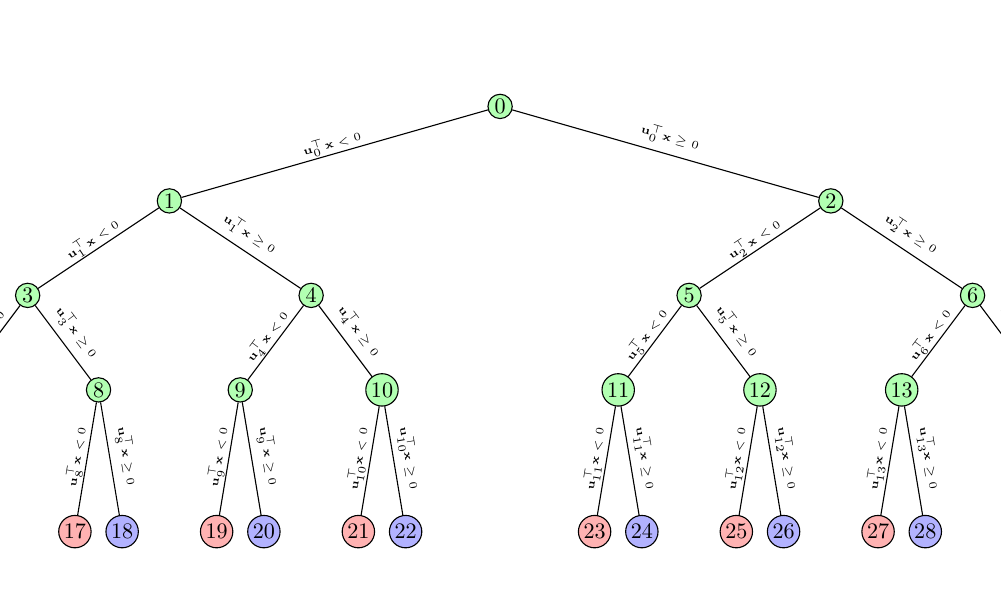
\begin{tikzpicture}[every node/.style={circle,draw,minimum size=10pt,inner sep=1pt, scale=0.8}]

\path[use as bounding box] (-6, -6) rectangle (6, 1);
\begin{scope}[shift={(-0,0)}, scale=0.6]
% Level 0 (root)
\node[fill=green!30] (n0) at (0,0) {0};

% Level 1
\node[fill=green!30] (n1) at (-7,-2) {1};
\node[fill=green!30] (n2) at (7,-2) {2};

% Level 2
\node[fill=green!30] (n3)  at (-10,-4) {3};
\node[fill=green!30] (n4)  at (-4,-4) {4};
\node[fill=green!30] (n5)  at (4,-4) {5};
\node[fill=green!30] (n6)  at (10,-4) {6};

% Level 3
\node[fill=green!30] (n7)  at (-11.5,-6) {7};
\node[fill=green!30] (n8)  at (-8.5,-6) {8};
\node[fill=green!30] (n9)  at (-5.5,-6) {9};
\node[fill=green!30] (n10) at (-2.5,-6) {10};
\node[fill=green!30] (n11) at (2.5,-6) {11};
\node[fill=green!30] (n12) at (5.5,-6) {12};
\node[fill=green!30] (n13) at (8.5,-6) {13};
\node[fill=green!30] (n14) at (11.5,-6) {14};

% Level 4 (leaves)
\node[fill=red!30] (n15)  at (-12,-9) {15};
\node[fill=blue!30] (n16)  at (-11,-9) {16};
\node[fill=red!30] (n17)  at (-9,-9) {17};
\node[fill=blue!30] (n18)  at (-8,-9) {18};
\node[fill=red!30] (n19)  at (-6,-9) {19};
\node[fill=blue!30] (n20)  at (-5,-9) {20};
\node[fill=red!30] (n21)  at (-3,-9) {21};
\node[fill=blue!30] (n22)  at (-2,-9) {22};
\node[fill=red!30] (n23)  at (2,-9) {23};
\node[fill=blue!30] (n24)  at (3,-9) {24};
\node[fill=red!30] (n25)  at (5,-9) {25};
\node[fill=blue!30] (n26)  at (6,-9) {26};
\node[fill=red!30] (n27)  at (8,-9) {27};
\node[fill=blue!30] (n28)  at (9,-9) {28};
\node[fill=red!30] (n29)  at (11,-9) {29};
\node[fill=blue!30] (n30)  at (12,-9) {30};

% Edges
\foreach \i in {0,...,14} {
   \pgfmathtruncatemacro\leftchild{2*\i+1}
   \pgfmathtruncatemacro\rightchild{2*\i+2}
   \draw (n\i) -- (n\leftchild) node[midway, sloped, anchor=south, yshift=-11pt, draw=none] {\tiny{$\bu_{\i}^\top \x <0$}};
   \draw (n\i) -- (n\rightchild) node[midway, sloped, anchor=north, allow upside down, yshift=23pt, draw=none] {\tiny{$\bu_{\i}^\top \x\geq0$}};
}
\end{scope}
\end{tikzpicture}

\caption{The decision tree with depth $D=4$ has its decision nodes shaded green. Label nodes colored red have $y^*=+1$ and label nodes colored blue have $y^*=-1$.}
\label{fig:ODT}
\end{figure}

Let $\Gamma$ denote the set of root-to-label paths in the ODT. Each $\gamma \in \Gamma$ is a $(D+1)$-tuple, and is associated with a sign vector $\tau(\gamma)\in\{+1,-1\}^D$ recording the sequence of left/right decisions. For example, in a depth-$4$ tree, the path $\gamma=(0,1,3,7,15)$ has $\tau(\gamma)=(-1,-1,-1,-1)$ and label $y^*(\gamma)=+1$.

\begin{equation}
\begin{aligned}
y^*(\x) = \sum_{\gamma \in \Gamma} y^*(\gamma)\prod_{p=1}^D \mathbf{1}\!\left(\tau_p \, \bu_{\gamma_p}^\top \x > 0\right),
\end{aligned}
\label{eqn:ODT_defn}
\end{equation}
where $\tau_p$ denotes the $p$-th entry of $\tau(\gamma)$. By construction, exactly one path in $\Gamma$ contributes non-zero mass for any given $\x$.

\subsection{The Deep Linearly Gated Network Architecture Setting}
\label{sec:DLGN_intro}

The Deep Linearly Gated Network (DLGN) is defined as a sum of products of sigmoidal gates applied to linear functions:
\begin{equation}
    \hat y(\x) = \sum_{\pi \in \Pi} a_\pi \prod_{\ell=1}^L \phi(\w_{\pi,\ell}^\top \x),
    \label{eq:DLGN_path_dec}
\end{equation}
where $\Pi$ is a discrete index set, $L$ is the number of layers, and $\phi:\R\to[0,1]$ is a scaled sigmoid, $\phi(u)=1/(1+\exp(-\beta u))$. The vectors $\w_{\pi,\ell}$ and coefficients $a_\pi$ are the trainable parameters.

To connect this model to standard deep architectures, \citet{Banerjee+25} take $\Pi=[M]^L$, corresponding to all paths through a network with $L$ hidden layers and $M$ neurons per layer. The parameterization is then shared across paths: for $\pi=(m_1,\ldots,m_L)\in[M]^L$, the gate vector at layer $\ell$ depends only on $m_\ell$, i.e. $\w_{\pi,\ell}=\w_{m_\ell,\ell}$. The path coefficient $a_\pi$ is taken to be the product of edge weights along $\pi$ in an associated deep linear network,
$
a_\pi = \prod_{\ell=2}^L a_{\ell,m_{\ell-1},m_\ell}.
$

This shared parameterization still allows the model output to be evaluated in $O(M^2L)$ time without explicitly summing over all $M^L$ paths.

\section{Learning Dynamics of Single-Path DLGN}
\label{sec:single-path-DLGN}

This model cannot fit the full ODT-labeled task, but it can capture a single ODT path and is therefore a useful setting for isolating the mechanism of interest. We now analyze how gradient descent on this model interacts with the ODT structure.
\[
\hat y(\x; a, W) = a \prod_{\ell=1}^L \phi(\w_\ell^\top \x),
\]
with parameters $a \in \R$ and $\w_1,\ldots,\w_L \in \R^d$. For convenience, we concatenate the $L$ gating vectors into $W \in \R^{Ld}$, and let $P_\ell:\R^d\to\R^{Ld}$ denote the operator that writes a vector into the $\ell$-th $d$-dimensional block and zeros elsewhere.

This model cannot in general fit the ODT-labeled data exactly, but its form suggests that it can effectively capture one path of the ODT labeling function. We now analyze how gradient descent on this model interacts with the ODT structure.

\subsection{Lens and blinders}

Our analysis starts from the loss gradient with respect to a single gating vector $\w_k$. For a data point $(\x,y^*)$ with $y^*$ given by \eqref{eqn:ODT_defn}, the logistic loss and its gradient are
\begin{align}
\mathcal{L}(\hat y(\x))
&= \log\!\big(1+\exp(-y^* \hat y(\x))\big), \nonumber \\
-\nabla_{\w_k} \mathcal{L}
&= \E\!\left[ \underbrace{\sigma(-y^* \hat y(\x))}_{\text{Residue}}
 \underbrace{\Lambda_k(\x)}_{\text{Lens}}
 \underbrace{\phi'(\w_k^\top \x)}_{\text{Blinder}} \, y^* a \x \right],
\label{eqn:ResidueLensBlinder}
\end{align}
where $\Lambda_k(\x) = \prod_{\kappa \neq k} \phi(\w_\kappa^\top \x)$.

Thus the update to $\w_k$ is a Perceptron-type update on the whole training set, with each example $(\x,y^*)$ weighted by the product of residue, lens, and blinder terms. From this viewpoint, $\w_k$ is trained as a separator on data reweighted by a lens formed by the other layers, while simultaneously serving as a component of the lens that shapes the gradients of those layers.

When the lens emphasizes certain regions of input space, the resulting gradient can have a strong component along feature directions that do not dominate globally, such as the ODT root direction $\bu_0$. This creates a positive-feedback mechanism in which movement of one layer can encourage other layers to move toward complementary task-relevant features.

\subsection{Second-order analysis}
\label{sec:second_order_analysis}

To analyze feature learning, we study how the NTK features change during training, which corresponds to a second-order analysis of the loss. Specializing this analysis to ODT-labeled data, we show how the interaction between the “lens” and “separator” roles of a neuron $\w_k$ can encourage the model to acquire ODT decision vectors that are initially absent from the gradient.

\begin{theorem}[Hierarchy-seeking lens]
\label{thm:second_order_lens}
Let $\h,\z \in \R^d$. Let $0<a<1$ and $k\neq \ell$. Assume $\w_\lambda^\top \h = \w_\lambda^\top \z = 0$ for all $\lambda \in [L]$. Then the change in the gradient of $\mathcal{L}$ with respect to $\w_k$ in direction $\z$ as $\w_\ell$ moves in direction $\h$ satisfies
\begin{align*}
\lim_{\epsilon \to 0} \frac{1}{\epsilon} \Big[
 -\nabla_{\w_k} \mathcal{L}(W + \epsilon P_\ell(\h))
 + \nabla_{\w_k} \mathcal{L}(W) \Big]\cdot \z > 0,
\end{align*}
for the choice $\z = s \bu_i$ and $\h = \bu_j$, where $j\in\{N/2,\ldots,N\}$ is a leaf node of the ODT and $i$ is any ancestor of $j$. The scalar $s=+1$ if $j$ lies in the left subtree of $i$ and $s=-1$ otherwise. The same inequality holds when $\h$ and $\z$ are swapped.
\end{theorem}

As one concrete consequence, if $\w_\ell$ moves along $-\bu_j$ for some leaf node $j$ on the left of the root node $0$, then $\w_k$ is pushed along $-\bu_0$. This formalizes a tendency of gradient descent in this model: movement of one neuron along a leaf direction can increase the incentive for another neuron to move along an ancestor direction. In high-dimensional settings where the initial $\w_k$ are nearly orthogonal to all ODT directions, the raw gradient has negligible component along internal-node directions such as $\bu_0$, so this second-order effect provides a concrete route by which such features can enter the dynamics.

Under a symmetric initialization such as $W=0$ with $a>0$, gradient descent reaches a saddle point $W^*$ where each of the $L$ neurons takes the same vector $\w^* = c\sum_{j} -\bu_j$, with $j$ ranging over leaf indices $N/2$ to $N$. The second-order dynamics captured in Theorem~\ref{thm:second_order_lens} imply that small asymmetric perturbations away from this saddle can trigger a positive feedback loop in which different layers specialize toward different ODT directions. We illustrate this effect with an explicit initialization in Section~\ref{sec:single_trajectory}.

Second-order effects can also produce undesirable couplings.

\begin{theorem}[Self-opposing lens]
\label{thm:second_order_backlash}
Let $\h \in \R^d$ be orthogonal to all ODT decision vectors $\bu_i$ for $i \in \{0,1,\ldots,N\}$. Assume $\w_\lambda \cdot \h = 0$ for all $\lambda \in\{1,\ldots,L\}$ and $\w_\lambda \cdot \bu_j = 0$ for all $\lambda$ and all $j \in \{N/2,\ldots, N\}$. Then the change in the gradient of $\mathcal{L}$ with respect to $\w_k$ along $\h$ as $\w_\ell$ (for some $\ell \neq k$) moves along $-\h$ satisfies
\begin{align*}
\lim_{\epsilon \to 0} \frac{1}{\epsilon} \Big[
 -\nabla_{\w_k} \mathcal{L}(W + \epsilon P_\ell(\h))
 + \nabla_{\w_k} \mathcal{L}(W) \Big]\cdot (-\h) > 0.
\end{align*}
\end{theorem}

Informally, if some neuron $\w_\ell$ is perturbed along a direction $\h$ that is orthogonal to all ODT decision vectors, then other neurons $\w_k$ tend to move along $-\h$, increasing the magnitude of both $\h$ and $-\h$ components across layers. In other words, neurons can end up trying to correct each other’s spurious movements and, in doing so, reinforce structure in directions that are irrelevant for generalization. This phenomenon becomes more pronounced in the multi-path DLGN, where many such couplings can interact; we return to this point in Section~\ref{sec:gating_regularization}.

Theorems~\ref{thm:second_order_lens} and \ref{thm:second_order_backlash} are derived under orthogonality assumptions (in particular, $d \gg D$ so that random initial weights are likely to be nearly orthogonal to all $\bu_i$). The relevant second-order quantities are continuous in $W$, so the qualitative effects persist under small deviations from strict orthogonality. In our experiments, we use these theorems as a guide to interpret and predict training trajectories, rather than as a complete description of the dynamics at all times.

\subsection{Trajectory analysis for a chosen initialization}
\label{sec:single_trajectory}

\begin{figure}
\includegraphics[width=1\linewidth]{figs/Single_path_DLGN/parameter_trajectory_0178_400epochs.pdf}
\includegraphics[width=1\linewidth]{figs/Single_path_DLGN/gradient_trajectory_0178_400epochs.pdf}
\caption{Parameter and gradient trajectories for a single-path DLGN under gradient descent.}
\label{fig:single_trajectory_0178}
\end{figure}

We now illustrate the above mechanisms with an explicit trajectory. We consider a depth-$D=4$ ODT label function and a single-path DLGN with $L=D=4$, fix $a=1$, and study the evolution of the gating vectors $\w_\ell$ under gradient flow. The same construction can be extended to deeper trees and DLGNs.

Because $a>0$, the model can achieve non-trivial log loss (values below $\log 2$) only on positively labeled points, i.e. data reaching label nodes $15,17,\ldots,29$, which all lie on the left side of their parents. With initialization $W=0$ and $a>0$, symmetry implies that gradient descent pushes each $\w_k$ along $\sum_j -\bu_j$, where $j$ ranges over leaf indices $N/2$ to $N$, until it reaches the saddle point $W^*$; the gradient has no component along other directions at this point.

We now perturb this initialization slightly in a direction suggested by Theorem~\ref{thm:second_order_lens}. Let
\[
\w_1 = 0,\quad
\w_2 = -\epsilon \bv,\quad
\w_3 = -\epsilon \bv - \epsilon \bu_7,\quad
\w_4 = -\epsilon \bv - \epsilon \bu_8,
\]
for some small $\epsilon>0$ and $\bv = \bu_7+\bu_8+\bu_9+\bu_{10}$. The resulting parameter and gradient trajectories are shown in Figure~\ref{fig:single_trajectory_0178}. From the perspective of $\w_1$, the other layers have moved along $-\bu_7,-\bu_8,-\bu_9,-\bu_{10}$, so Theorem~\ref{thm:second_order_lens} predicts an increased push on $\w_1$ toward $-\bu_0$. Swapping the roles of $\h$ and $\z$ in the theorem implies that movement of $\w_1$ toward $-\bu_0$ increases the tendency of the other layers to move along leaf-node directions, closing a feedback loop. The small additional perturbations of $\w_3$ and $\w_4$ along $-\bu_7$ and $-\bu_8$ similarly induce a tendency for $\w_2$ to move along $-\bu_1$, which becomes pronounced once $\w_1$ has moved sufficiently toward $-\bu_0$.

At the same time, Theorem~\ref{thm:second_order_backlash} implies a self-inhibitory effect: movement of $\w_1$ toward $-\bu_0$ discourages other neurons from doing the same, and indeed the other layers briefly move slightly along $+\bu_0$ around the time $\w_1$ experiences its largest push toward $-\bu_0$. Although all neurons initially have an increased tendency to move toward $-\bu_0$, this effect is strongest for $\w_1$.

Figure~\ref{fig:single_trajectory_0178} shows that the first $\approx 10$ epochs move the parameters from the perturbed initialization to the saddle $W^*$. The influence of the second-order dynamics described above becomes visible thereafter: from roughly epoch $10$ to $50$, the gradient component of $\w_1$ along $-\bu_0$ strengthens; from epoch $50$ to $90$, the gradient component of $\w_2$ along $-\bu_1$ increases; and $\w_3,\w_4$, which were initially biased toward $-\bu_7$ and $-\bu_8$, continue to grow along those directions. The convergent solution (up to scaling) is well approximated by
\[
\w_1 \approx -\bu_0,\quad
\w_2 \approx -\bu_1,\quad
\w_3 \approx -\bu_7 + 0.3\,\bu_3,\quad
\w_4 \approx -\bu_8 - 0.3\,\bu_3,
\]
as shown in Appendix Figure~\ref{fig:full_trajectory}. This corresponds to a superposition of two adjacent positively labeled ODT paths, e.g. $(-\bu_0,-\bu_1,-\bu_7,-\bu_3)$ and $(-\bu_0,-\bu_1,+\bu_3,-\bu_8)$.

For $D=L=4$, there are four such solutions, corresponding to the leaf pairs $(7,8)$, $(9,10)$, $(11,12)$, and $(13,14)$. Permutation invariance across the $L$ layers yields $4!=24$ configurations per pair, for a total of $96$ solutions in parameter space (in general, $2^{D-2} D!$ when $D=L$). Small perturbations around $W=0$ can be constructed to reach any of these solutions under gradient descent.

We represent these solutions compactly by a $D$-tuple recording which ODT direction each neuron aligns with most strongly. For a solution $\tilde W \in \R^{D\times d}$, define $\upsilon(\tilde W) \in \{0,1,\ldots,2^D-2\}^D$ by
\[
\upsilon_\ell(\tilde W) = \arg\max_{i \in \{0,\ldots,2^D-2\}} |\w_\ell \cdot \bu_i|.
\]
For the trajectory in Figure~\ref{fig:single_trajectory_0178}, we obtain $\upsilon(\tilde W) = [0,1,7,8]$.

\subsection{Solution prediction from random initialization}
\label{sec:trajectory_prediction}

The construction above shows that carefully designed perturbations can steer gradient descent toward any of the $2^{D-2}D!$ canonical solutions. For typical random initializations, however, the perturbations from $0$ need not align perfectly with a single canonical pattern, and several solutions may be supported simultaneously. Assuming that gradient descent converges to one of the $96$ solutions, we ask: which one does a given initialization select?

We do not have a closed-form answer, but we can build a heuristic score that uses Theorems~\ref{thm:second_order_lens} and \ref{thm:second_order_backlash} to estimate the support an initialization $W(0)$ gives to each solution. The construction, detailed in Appendix~\ref{sec:appendix_heuristic_score}, combines three terms: a proximity term measuring how close $W(0)$ is to the solution, a hierarchy-seeking term weighted by $c_{\text{HS}}\ge 0$, and a self-opposing term weighted by $c_{\text{SO}}\ge 0$.

We run gradient descent for the single-path DLGN with $2000$ different initializations, each evaluated on $5$ independently sampled datasets to separate initialization effects from finite-data noise. For $368$ initializations, the convergent solution is stable across datasets, and we treat these as “deterministic” initializations. We search $c_{\text{HS}}, c_{\text{SO}} \in \{0.0,0.1,\ldots,0.9\}$, and find that the best-performing pair $(c_{\text{SO}},c_{\text{HS}})=(0.7,0.4)$ correctly predicts the converged solution for $179$ out of $368$ deterministic initializations, corresponding to $49\%$ accuracy in a $96$-class prediction problem.

A simple baseline that predicts the solution closest (in parameter space) to the initialization corresponds to $(c_{\text{SO}},c_{\text{HS}})=(0,0)$ and attains only $13\%$ accuracy. Moreover, the best achievable accuracy when forcing $c_{\text{HS}}=0$ is $28\%$, and when forcing $c_{\text{SO}}=0$ is $36\%$. Both the hierarchy-seeking and self-opposing terms are therefore important for predictive power in this heuristic, providing quantitative support for our viewpoint in the single-path DLGN setting.



\section{Learning Dynamics of Multi-Path DLGN}
\label{sec:multi-path-DLGN}

\begin{figure*}
\centering
\includegraphics[width=0.48\linewidth, trim={0 0 0 0.9cm},clip]{figs/Multi_path_DLGN/DLGN_one_phase_scatter.pdf}
\includegraphics[width=0.48\linewidth, trim={0 0 0 0.9cm},clip]{figs/Multi_path_DLGN/DLGN_2phase_phase1_scatter.pdf}
\caption{Gating norms vs.\ cosine similarity to ODT vectors for a 5-layer DLGN with $M=16$: (a) standard log-loss training, (b) with an additional $L_2$ penalty on gating vectors.}
\label{fig:norms_cosine_scatter_DLGN}
\end{figure*}

We now turn to the more practical multi-path DLGN with $M>1$. With $M=1$, the model can at best capture data entering one leaf node of the ODT, achieving low loss on only a $2^{-D}$ fraction of examples and close to random performance on the rest. Wider DLGNs do not suffer from this limitation.

Throughout this section we consider $d=100$, depth-$5$ ODT-labeled data, and a 5-layer DLGN with $M=16$ neurons per layer. In this setting, the DLGN achieves low training loss and low test error on the full dataset, whereas linear, kernel, and standard tree-based baselines remain above $30\%$ test error (see Appendix~\ref{app:performance}).

\subsection{Effect of gating regularization}
\label{sec:gating_regularization}

We first train the DLGN by minimizing the log loss over both path coefficients $a$ and gating vectors $\w$ using a standard gradient-based optimizer. In this regime, the train loss decreases from $\log 2 \approx 0.69$ at initialization to about $0.05$, and the test error drops from roughly $50\%$ to about $17\%$. For a typical architecture/dataset combination this would often be considered satisfactory, with further improvement delegated to hyperparameter tuning.

In our ODT setting, however, we can inspect learning behavior more directly using the known ODT decision vectors $\bu_j$. Ideally, as training progresses, gating vectors $\w_{m,\ell}$ that grow in norm should also align with some ODT direction $\bu_j$, since any component orthogonal to all $\bu_i$ does not help fit the target function. Figure~\ref{fig:norms_cosine_scatter_DLGN}(a) shows, at the end of standard training, the norm of each gating vector versus its maximum cosine similarity with any ODT direction. While the initialization cloud sits around $(0.6,0.25)$ with no structure, after training we see many high-norm gating vectors that remain poorly aligned with all ODT directions. This suggests that a significant fraction of capacity is devoted to directions that are not directly related to the ODT structure.

Motivated by the self-opposing behavior in Theorem~\ref{thm:second_order_backlash}, where movement along spurious directions can propagate across layers, we explore a simple modification: adding an $L_2$ penalty on gating norms to the loss. This penalty is not primarily intended as a conventional regularizer for test performance, but as a way to discourage large-norm components in directions that are not supported by the ODT features, thereby altering the optimization landscape. As shown in Figure~\ref{fig:norms_cosine_scatter_DLGN}(b), training with this penalty leads to a markedly different outcome: almost all large-norm gating vectors align closely with some ODT decision vector.

The $L_2$ penalty, however, also limits the norms that gating vectors can achieve along ODT directions and slightly reduces attainable performance: in this regime the final training loss bottoms out around $0.03$, with test error near $13\%$. To retain the alignment benefits while allowing larger norms, we adopt a two-phase procedure. We first train with the $L_2$ penalty as above, then restart training from the convergent solution with the penalty removed. At the restart, we additionally prune gating vectors whose norms fall below a small threshold by setting them to zero and keeping them fixed in the second phase. This pruning step is motivated by Figure~\ref{fig:norms_cosine_scatter_DLGN}(b), which suggests that most useful gating vectors can be identified by their norms.

This two-phase strategy further reduces test error to about $6\%$ in our example. Averaging over 10 random seeds, we observe the following pattern: standard log-loss training yields $17.8\%\pm0.7\%$ test error; adding gating regularization alone improves this to $13\%\pm0.7\%$; restarting from the regularized solution without further regularization yields $8.9\%\pm0.7\%$; and adding pruning between the two phases attains $6\%\pm0.7\%$ test error. These results are consistent with the view that second-order interactions along irrelevant directions can produce undesirable behavior, and that shaping the gating norms can help mitigate this in the multi-path setting.

\subsection{Hierarchical feature emergence}
\label{sec:hierarchical_feature_emergence}

Theorem~\ref{thm:second_order_lens} suggests a hierarchical preference: random motion of a gating vector along any leaf-node direction tends to enhance movement along the root direction $\bu_0$, whereas similar second-order effects for deeper internal nodes require more specific conditions. The trajectory in Figure~\ref{fig:single_trajectory_0178} reflects this, with gating vectors first moving along the ODT root and then progressively along its children.

A similar pattern appears in the multi-path DLGN. We define the \emph{capture epoch} of an ODT direction $\bu_j$ as the first epoch at which there exists a gating vector with norm exceeding a fixed threshold (e.g.\ $>2.5$) and cosine similarity above a fixed threshold (e.g.\ $>0.8$) to $\bu_j$. Figure~\ref{fig:DLGN_ReLU_Hierarchical_feature_emergence}(a) shows these capture epochs for all ODT nodes when training a 5-layer DLGN with an $L_2$ penalty on the gating vectors from a random initialization. We observe a clear trend in which parent nodes tend to be captured earlier than their children, providing an empirical notion of hierarchical feature emergence consistent with the single-path analysis.

In the next section, we examine whether a related hierarchy is visible in standard ReLU networks as well.

\begin{figure}
\includegraphics[width=0.5\textwidth, trim={0 0 0 1cm},clip]{figs/Multi_path_DLGN/DLGN_phase1_odt_hit_epoch_trees_5178.pdf}
\includegraphics[width=0.5\textwidth, trim={0 0 0 1cm},clip]{figs/ReLU_3layer/relu_odt_capture_epochs_6178.pdf}
\caption{ODT node capture epochs for a depth-5 ODT: (a) across all gating vectors in a 5-layer DLGN, (b) across first-layer weight vectors in a 3-layer ReLU network.}
\label{fig:DLGN_ReLU_Hierarchical_feature_emergence}
\end{figure}






\section{ReLU evidence and broader interpretation}


While our theoretical results are proved for the DLGN, our experiments suggest that related phenomena also appear in ReLU networks. On the same ODT dataset, ReLU networks with two or more hidden layers (three or more weight matrices) achieve performance comparable to DLGNs and exhibit a similar hierarchical feature-emergence pattern. Figure~\ref{fig:DLGN_ReLU_Hierarchical_feature_emergence}(b) shows the capture epochs of ODT node vectors by the first layer of a ReLU network; the order of emergence closely resembles that observed in DLGNs.

We also perform intervention experiments in which gradient updates for the first layer weights of the  are projected onto the orthogonal complement of a chosen ODT direction $\bu_j$ during training. In these ReLU settings, such projections typically degrade final performance and substantially reduce alignment with ODT directions under the subtree of $j$, indicating that suppressing an internal-node direction can hinder the learning of its descendants. These observations are consistent with a hierarchical feature-discovery process in which internal features facilitate the acquisition of more local descendant features.

Viewed more broadly, the ODT setting can be interpreted through the concept of a \emph{scope of discontinuity}: the root node $0$ is more prominent than its child node $1$ because flipping the sign of $\x\cdot\bu_0$ would change labels for half the data, whereas flipping the sign of $\x\cdot\bu_1$ affects only a quarter. This notion of scope is tied to the labeling function rather than to the specific tree construction, and may be adaptable to more general settings where label changes concentrate along a hierarchy of increasingly localized discontinuities.

Throughout, the multiplicative cross-layer interactions in gradient computation act as an effective weighting mechanism from the viewpoint of each layer, potentially creating a positive feedback loop between the two roles of individual neurons: fitting the currently weighted data and helping shape the data seen by other neurons. Our DLGN analysis makes this structure explicit and tractable, but the underlying multiplicative dependence between layers is shared by many gated architectures, including ReLU networks. We view this as a plausible narrative for feature learning beyond 





\section{Conclusion}

This paper studied a mechanistic lens/separator view of feature learning in gated deep networks through the analytically transparent DLGN--ODT setting. In this view, individual neurons both fit the currently weighted data and help determine the effective weighting seen elsewhere in the network. 

Our single-path analysis identified two competing second-order effects in gradient descent: a hierarchy-seeking effect that can promote movement toward task-relevant internal features, and a self-opposing effect that can amplify movement along spurious directions. In wider DLGNs, these ideas help interpret both the emergence of ODT-aligned features and the optimization behavior that motivates regularization and two-phase training. We also observed related hierarchical feature-emergence patterns in ReLU networks, together with intervention results consistent with the proposed mechanism.

While our formal guarantees are restricted to the DLGN--ODT setting, the results suggest a broader connection between multiplicative cross-layer structure, gradient-based optimization, and hierarchical feature discovery. We hope this viewpoint provides a useful starting point for a more general theory of feature learning in deep networks.

\small
\bibliographystyle{plainnat}
\bibliography{References_NeurIPS_2026}
\normalsize

\section{Appendix}
\subsection{Notations}
\begin{table}[]
    \centering
    \caption{Table of notations}
    \begin{tabular}{c|c}
    Variable and domain & Meaning \\ \hline
    $d$ & Data dimension \\
    $D$ & Depth of ODT tree \\
    $L$ & \# of hidden layers in model  \\
    $\mathcal{L}$ & Log loss for binary classification \\
    $M$ & \# of neurons per hidden layer  \\
    $i,j, \iota, \zeta \in \{0,1,\ldots,N\}$  & ODT decision node indices, $N=2^D-2$ \\
    $\mu, \nu \in \{N+1,\ldots,2N+2\}$ & ODT label node indices \\
    $p,q \in \{0,1,2,\ldots,D\}$ & ODT depth indices \\
    $k,l,\kappa,\lambda \in \{1,2,\ldots,L\}$ & DLGN Model layer indices  \\
    $m \in \{1,2,\ldots,M\}$ & Neuron index \\ 
    $\pi \in \Pi=[M]^L$ & DLGN path index \\
    $\gamma \in \Gamma \subseteq \{0,\ldots,2N+2\}^{D+1}$ & ODT Path \\
    $\gamma(\x)$ & ODT path traversed by point $\x$ \\
    $\sigma(a)$ & $1/(1+\exp(-a))$ \\
    $\phi:\R\>[0,1]$ & Sigmoidal function. \\
    $\tau \in \{+1,-1\}^D$ & Sequence of left/right decisions \\
    $\text{lev(i)} \in \{0,\ldots,D\}$ & Distance of node $i$ from $0$ in the ODT \\
    $\text{par}(i) \in \{0,1,\ldots,N \}$ & Parent of node $i$ \\
    $\text{anc}(i) \subseteq \{0,1,\ldots,N \}$ & Ancestors of node $i$ \\
    $\bv,\h,\z$ & Some vectors in $\R^d$ \\
    $\bu_j \in \R^d$ & ODT decision vector for node $j$ \\
    $\w_\ell \in \R^d$ & DLGN parameter in layer $\ell$
    \end{tabular}
    
    
    \label{tab:notations}
\end{table}


% \section{ReLU setup}

%Consider a standard ReLU network with $L$ hidden layers and $M$ hidden nodes per layer. With activations $\x^\ell =\psi(W^\ell \x^{\ell-1})$, where $\x^0 = \x \in \R^d$ and the output of the model $\hat {y}(\x) = W^{L+1} \cdot \x^L$. Here $\psi$ is the ReLU function. Here $W^1 \in \R^{M \times d}$ and $W^2,\ldots,W^L \in \R^{M \times M}$ and $W^{L+1} \in \R^{1\times M}$. Let $\g^1, \g^2,\ldots, \g^L$ be the pre-activations (i.e. $\psi(\g^\ell) = \x^\ell$) for the hidden layers. Let $\blambda^1, \ldots, \blambda^L \in \{0,1\}^M$ denote the activation status of the hidden neurons, i.e. $\blambda^\ell = \1(\g^\ell \geq 0)$. Note that $\x^\ell, \g^\ell, \blambda^\ell$ are all functions of the input $\x$. The ReLU network also admits a path decomposition of the form of Equation \ref{eq:DLGN_path_dec}, i.e.
%\begin{equation}
%    \hat y(\x) = \sum_{\pi \in [M]^L} \left( W^1_{m_1} \cdot \x \right) \prod_{\ell=1}^L \lambda^\ell_{m_\ell}(\x)   \left(W^{\ell+1}_{m_{\ell+1}, m_\ell}\right)
%\end{equation}
%where $\pi = (m_1, m_2,\ldots,m_L)$, and $m_{L+1}=1$ as convention. The main difference between ReLU and DLGN is that the gating functions $\lambda^\ell_{i_\ell}$ for the ReLU network are significantly more complex than the half-spaces for the DLGN (with $\phi(u)$ being the step function). 
%
%Despite this complication, one can show a similar result as the Hierarchy-seeking and self-opposing lens theorems for the DLGN.
%
%\begin{theorem}
%    
%\end{theorem}

For any vectors $\h,\z$, We use both $\h \cdot \z$ and $\h^\top \z$ to both mean the dot product, and will use $\h \cdot \z$, whenever it is inconvenient to use $\h^\top \z$. Table \ref{tab:notations} lists all the notations used in the paper.


\subsection{Proof for Theorem \ref{thm:second_order_lens}}
\begin{theorem*}
Let $\h, \z$ be vectors in $\R^d$. Let $0<a<1, k\neq \ell$. Let $\w_\lambda^\top \h = \w_\lambda^\top \z = 0$ for all $\lambda$. The change in gradient of $\mathcal{L}$ w.r.t. $\w_k$ along $\z$,   as $\w_\ell$, moves along $\h$ satisfies
% \[
%  -\h^\top  \big[\nabla^2_{\ell,k} L(W) \big] \z =  \lim_{\epsilon \> 0} \frac{1}{\epsilon} \bigg[ -\nabla_{\w_k} L(W + \epsilon P_\ell(\h)) \cdot \z  + \nabla_{\w_k} L(W) \cdot \z \bigg] > 0
% \]

\begin{align*}
\lim_{\epsilon \to 0} \frac{1}{\epsilon} \bigg[ 
 -\nabla_{\w_k} \mathcal{L}(W + \epsilon P_\ell(\h))  
 + \nabla_{\w_k} \mathcal{L}(W)  \bigg]\cdot \z > 0
\end{align*}

where $\z= s \bu_i, \h = \bu_j$,  $j\in\{N/2,\ldots,N\}$ is a leaf node of the ODT, and $i$ is any ancestor of $j$. The scalar $s=+1$ if $j$ is in the left sub-tree of $i$ and $-1$ otherwise. The above inequality also holds when $\h$ and $\z$ are swapped.
\end{theorem*}

\label{app:second_order_lens}
\begin{proof}
Without loss of generality, let $j=N/2$. Let $\gamma(\x) \in \{0,1,\ldots,2N+2\}^{D+1}$ be the path traversed in the ODT by data point $\x$. Its $D$-th element $\gamma_D(\x)$ gives the leaf decision node, and its $D+1$-th element $\gamma_{D+1}(\x)$ gives the label node. The label $y(\x) =  +1$ if $\gamma_{D+1}(\x)$ is odd, and $-1$ otherwise. Let $\epsilon>0$ be an arbitrarily small number. All expressions involving $\epsilon$ below ignore quadratic and higher terms.

Let $\alpha(\x) = \frac{\phi(\w_{\ell} ^\top \x + \epsilon \h^\top \x)}{\phi(\w_{\ell} ^\top \x)} = 1+\frac{\epsilon \h^\top\x \phi'(\w_\ell^\top \x)}{\phi(\w_\ell^\top \x)}$.
\begin{align}
\lefteqn{-\nabla_{\w_k} \mathcal{L}(W + \epsilon P_\ell(\h)) \cdot \z } \nonumber \\
&= 
\E_{\x} \left[ \sigma (-y^*(\x) \hat y(\x)\alpha(\x)) \Lambda_k(\x) \alpha(\x) \phi'(\w_k^\top \x) y^*(\x)a \x \cdot \z \right] \nonumber  \\
&= \frac{2}{2^D} \sum_{\iota = N/2}^{N}  \E_{\x} \left[ \sigma (-y^*(\x) \hat y(\x)\alpha(\x)) \Lambda_k(\x) \alpha(\x) \phi'(\w_k^\top \x) y^*(\x) a \x \cdot \z  \bigg{|} \gamma_{D}(\x) = \iota \right] \label{eq:second_order_eq1}
\end{align}
We will analyze the sum of these conditional expectation terms separately for each $\iota$. For each $\x'$, such that $\gamma_{D}(\x') = \iota $ and $\h^\top \x' > 0$ consider its reflection $\tilde \x$ along $\h = \bu_j$ i.e. $\tilde\x = (I-2 \bu_j \bu_j^\top)\x'$.  Let us consider a sum over just these two points (instead of an expectation over all $\x,y$).
\begin{align}
\lefteqn{\sum_{\x=\x',\tilde\x} \sigma (-y^*(\x) \hat y(\x)\alpha(\x)) \Lambda_k(\x) \alpha(\x) \phi'(\w_k^\top \x) y^*(\x)a \x \cdot \z } \nonumber  \\
&=
\sum_{\x=\x',\tilde\x} \left(\sigma(-y^*(\x) \hat y(\x))+\epsilon(-y^*(\x) \hat y(\x)) \sigma'(-y^*(\x) \hat y(\x))\frac{\h^\top \x \phi'(\w_\ell^\top \x)}{\phi(\w_\ell^\top \x)} \right) \nonumber \\ 
&\Lambda_k(\x) \left(1+\frac{\epsilon \h^\top\x \phi'(\w_\ell^\top \x)}{\phi(\w_\ell^\top \x)}\right) \phi'(\w_k^\top \x) y^*(\x) a \x \cdot \z \nonumber  \\
&= \sum_{\x=\x',\tilde\x} \sigma(-y^*(\x) \hat y(\x)) \Lambda_k(\x) \phi'(\w_k^\top \x) y^*(\x)a \x \cdot \z ~ +   \nonumber  \\
& \qquad \qquad \frac{\epsilon \h^\top\x \phi'(\w_\ell^\top \x)}{\phi(\w_\ell^\top \x)}\left( \sigma(-y^*(\x) \hat y(\x))- y^*(\x) \hat y(\x) \sigma'(-y^*(\x) \hat y(\x) \right)\Lambda_k(\x) \phi'(\w_k^\top \x) y^*(\x)a \x \cdot \z  \label{eq:second_order_eq1a} 
\end{align}
\textbf{Case 1}:  $\iota>N/2$.
As $\iota \neq j$, we have that $\tilde\x$ and $\x'$ share the same ODT path, i.e. $\gamma(\tilde\x) = \gamma(\x')$, and hence the same label $y^*(\x)$. As the weights $\w_\lambda$ and the vector $\z$ are all orthogonal to $\h = \bu_j$ , all terms except $\h^\top \x$ are the same for both $\x=\x'$ and $\x=\tilde\x$. Further,  $\h^\top \x' = -\h^\top \tilde \x$, thus making the second term in the above sum equal to zero. Thus Equation \ref{eq:second_order_eq1a} becomes
\begin{align}
\sum_{\x=\x',\tilde\x} \sigma (-y^*(\x) \hat y(\x)\alpha(\x)) \Lambda_k(\x) \alpha(\x) \phi'(\w_k^\top \x) y^*(\x)a \x \cdot \z 
&= \sum_{\x=\x',\tilde\x} \sigma(-y^*(\x) \hat y(\x)) \Lambda_k(\x) \phi'(\w_k^\top \x) y^*(\x)a \x \cdot \z \label{eq:second_order_eq2}
\end{align}


\textbf{Case 2:} $\iota = N/2$. 
As $\iota=j$, the point $\x'$ and $\tilde \x$ differ in their ODT paths -- one of them terminates in label node $N+1$ and the other terminates in label node $N+2$, and have different labels $y^*(\x)$. Note that $\z=s\bu_i$. Without loss of generality let $j$ be in the left sub-tree of $i$, and $s=+1$. Thus $\x.\z < 0$ for both $\x=\x'$ and $\x=\tilde \x$. Further, we have $\h = \bu_j$ where $j=N/2$ which is a leaf node, thus the label $y^*(\x)$ for both $\x=\x'$ and $\x = \tilde \x$ is simply $\text{sign}(-\h \cdot \x)$. Hence, $y^*(\x) \h^\top \x (\x.\z) > 0$.  Now note that as $0<a<1$ the value  $\hat y(\x)$ is also between $0$ and $1$. The term $\big(\sigma(-y^*(\x) \hat y(\x))- y^*(\x) \hat y(\x) \sigma'(-y^*(\x) \hat y(\x)\big)$ is clearly positive for $y^*(\x)=-1$. For $y^*(\x)=+1$, the term $\big(\sigma(-y^*(\x) \hat y(\x))- y^*(\x) \hat y(\x) \sigma'(-y^*(\x) \hat y(\x)\big)$ is also positive because $\sigma'(q)<\sigma(q)$ and $0<y^*(\x)\hat y(\x)<1$ Equation \ref{eq:second_order_eq1a} then becomes
\begin{align}
\sum_{\x=\x',\tilde\x} \sigma (-y^*(\x) \hat y(\x)\alpha(\x)) \Lambda_k(\x) \alpha(\x) \phi'(\w_k^\top \x) y^*(\x)a \x \cdot \z 
&>\sum_{\x=\x',\tilde\x} \sigma(-y^*(\x) \hat y(\x)) \Lambda_k(\x) \phi'(\w_k^\top \x) y^*(\x)a \x \cdot \z \label{eq:second_order_eq3}
\end{align}
Putting both the cases together, adding all the conditional expectation terms in Equation \ref{eq:second_order_eq1} using the inequalities in Equations \ref{eq:second_order_eq2} and \ref{eq:second_order_eq3}, we get
\begin{align*}
-\nabla_{\w_k} \mathcal{L}(W + \epsilon P_\ell(\h)) \cdot \z  
>
-\nabla_{\w_k} \mathcal{L}(W ) \cdot \z  
\end{align*}
This completes the proof for the main Theorem statement.
Now, consider the case when $\h$ and $\z$ are swapped. Let the $dL \times dL$ Hessian of $\mathcal L$ w.r.t all the gating vectors $\w_1, \ldots, \w_L$ be denoted by $H$. We have that 
\[\lim_{\epsilon \to 0} \frac{1}{\epsilon} \bigg[ 
 -\nabla_{\w_k} \mathcal{L}(W + \epsilon P_\ell(\h))  
 + \nabla_{\w_k} \mathcal{L}(W)  \bigg]\cdot \z  = -P_\ell(\h)^\top H P_k(\z).\] 
To prove the same for $\h$ and $\z$ swapped, requires just seeing that $P_\ell(\h)^\top H P_k(\z) = P_\ell(\z)^\top H P_k(\h)$, which is true by symmetry of $H$.
\end{proof}

\subsection{Proof for Theorem \ref{thm:second_order_backlash}}
\label{app:second_order_backlash}
\begin{theorem*}
Let $\h$ be a vector in $\R^d$ that is orthogonal to the ODT decision vectors $\bu_i$ for all $i \in \{0,1,\ldots,n\}$. 
% Let the lens for layer $k$ be at most mildly positively correlated with the label $y$, i.e. $\E[\Lambda_k(\x) y ] < \frac{1}{N}\E[\Lambda_k(\x)]$. 
Let $\w_\lambda \cdot \h = 0$ for all $\lambda \in\{1,\ldots,L\}$. Let $\w_\lambda \cdot \bu_j = 0$ for all $\lambda \in\{1,\ldots,L\}$ and $j \in \{N/2,\ldots, N\}$. The change in gradient of $\mathcal{L}$ w.r.t. $\w_k$ along $\h$  as $\w_\ell$ (for some $\ell \neq k$) moves along $-\h$ satisfies the following relation.

\begin{align*}
\lim_{\epsilon \to 0} \frac{1}{\epsilon} \bigg[ 
 -\nabla_{\w_k} \mathcal{L}(W + \epsilon P_\ell(\h))  
 + \nabla_{\w_k} \mathcal{L}(W)  \bigg]\cdot (-\h) > 0
\end{align*}
\end{theorem*}
\begin{proof}
Without loss of generality, we assume $a>0$. Similar arguments with the exact same conclusion follows for $a<0$ as well. Let $\epsilon>0$ be an arbitrarily small number. All expressions involving $\epsilon$ below ignore quadratic and higher terms. Let $\alpha(\x) = \frac{\phi(\w_{\ell} ^\top \x + \epsilon \h^\top \x)}{\phi(\w_{\ell} ^\top \x)} = 1+\frac{\epsilon \h^\top\x \phi'(\w_\ell^\top \x)}{\phi(\w_\ell^\top \x)}$ . 

\begin{align}
-\nabla_{\w_k} \mathcal{L}(W + \epsilon P_\ell(\h)) \cdot (-\h) 
&= 
\E_{\x} \left[ \sigma (-y^*(\x) \hat y(\x)\alpha(\x)) \Lambda_k(\x) \alpha(\x) \phi'(\w_k^\top \x) y^*(\x)a \x \cdot (-\h) \right] \nonumber  
\end{align}

For each $\x'$, such $y^*(\x')=1$ consider its reflection $\tilde \x$ along $\bu_{\zeta}$, where $\zeta = \gamma_D(\x')$ is the leaf node in the ODT corresponding to $\x'$. i.e. $\tilde\x = (I-2 \bu_\zeta \bu_\zeta^ \top)\x'$.  Let us consider a sum over just these two points (instead of an expectation over all $\x,y$). By construction, $y^*(\tilde \x)=-1$. 
\begin{align}
\lefteqn{\sum_{\x=\x',\tilde\x} \sigma (-y^*(\x) \hat y(\x)\alpha(\x)) \Lambda_k(\x) \alpha(\x) \phi'(\w_k^\top \x) y^*(\x)a \x \cdot (-\h) } \nonumber  \\
&=
\sum_{\x=\x',\tilde\x} \left(\sigma(-y^*(\x) \hat y(\x))-\epsilon y^*(\x)\hat y(\x) \sigma'(-y^*(\x) \hat y(\x))\frac{\h^\top \x \phi'(\w_\ell^\top \x)}{\phi(\w_\ell^\top \x)} \right) \nonumber \\
&\Lambda_k(\x) \left(1+\frac{\epsilon \h^\top\x \phi'(\w_\ell^\top \x)}{\phi(\w_\ell^\top \x)}\right) \phi'(\w_k^\top \x) y^*(\x)a \x \cdot (-\h) \nonumber  \\
&= \sum_{\x=\x',\tilde\x} \sigma(-y^*(\x) \hat y(\x)) \Lambda_k(\x) \phi'(\w_k^\top \x) y^*(\x)a \x \cdot (-\h) ~ +   \nonumber  \\
& \qquad \qquad \frac{\epsilon \h^\top\x \phi'(\w_\ell^\top \x)}{\phi(\w_\ell^\top \x)}\Big( \sigma(-y^*(\x) \hat y(\x))-y^*(\x)\hat y(\x) \sigma'(-y^*(\x) \hat y(\x)) \Big)\Lambda_k(\x) \phi'(\w_k^\top \x) y^*(\x) a \x \cdot (-\h)  \label{eq:second_order_backlash_eq1a} 
\end{align}
Expanding the second term above alone, we get
\begin{align}
\sum_{\x=\x',\tilde\x} \frac{ -\epsilon(\h^\top\x)^2 \phi'(\w_\ell^\top \x)}{\phi(\w_\ell^\top \x)}\Lambda_k(\x) \phi'(\w_k^\top \x) a\Big( \sigma(-y^*(\x) \hat y(\x))-y^*(\x)\hat y(\x) \sigma'(-y^*(\x) \hat y(\x)) \Big) y^*(\x) 
\label{eq:temp1}
\end{align}


Note that $\x$ and $\x'$ differ only in their projections along $\bu_\zeta$ which is orthogonal to all gating vectors $\w_\lambda$, and also $\h$. Due to orthogonality assumptions, the term $\frac{ -\epsilon(\h^\top\x)^2 \phi'(\w_\ell^\top \x)}{\phi(\w_\ell^\top \x)}\Lambda_k(\x) \phi'(\w_k^\top \x) a$ is the same for both $\x=\x'$ and $\x=\tilde \x$, and also negative. Analysing the remaining term, we get
\begin{align}
\sum_{\x=\x',\tilde\x}  \Big( \sigma(-y^*(\x) \hat y(\x))-y^*(\x)\hat y(\x) \sigma'(-y^*(\x) \hat y(\x)) \Big) y^*(\x)
&=
\sigma(-\hat y) - \hat y \sigma'(-\hat y) - \sigma(\hat y) - \hat y \sigma'(\hat y) \nonumber \\
&=  \sigma(-\hat y) - \sigma(\hat y) - 2 \hat y \sigma'(\hat y) < 0\label{eq:second_order_backlash_eq2}  
\end{align}
where we have used that $\hat y(\x') = \hat y (\tilde \x) = \hat y > 0$ and $y^*(\x') = - y^*(\tilde \x) = 1$.
Substituting Equation \ref{eq:second_order_backlash_eq2} into \ref{eq:temp1}, and the resulting term into Equation \ref{eq:second_order_backlash_eq1a}, we get
\begin{align}
\lefteqn{\sum_{\x=\x',\tilde\x} \sigma (-y^*(\x) \hat y(\x)\alpha(\x)) \Lambda_k(\x) \alpha(\x) \phi'(\w_k^\top \x) y^*(\x) a \x \cdot (-\h)} \nonumber \\ 
&>
\sum_{\x=\x',\tilde\x} \sigma (-y^*(\x) \hat y(\x)) \Lambda_k(\x) \phi'(\w_k^\top \x) y^*(\x)a \x \cdot (-\h)  \nonumber
\end{align}
and thus
\[
-\nabla_{\w_k} \mathcal{L}(W + \epsilon P_\ell(\h)) \cdot (-\h) 
>
-\nabla_{\w_k} \mathcal{L}(W) \cdot (-\h) 
\]
\end{proof}



\subsection{Single Path DLGN parameter trajectory}
As an extension to Figure \ref{fig:single_trajectory_0178} in Section \ref{sec:single_trajectory}, Figure \ref{fig:full_trajectory} shows the paramter trajectories when updated using gradient descent for 10000 epochs.

% \begin{figure*}
% \includegraphics[width=1.05\textwidth]{figs/Single_path_DLGN/parameter_trajectory_0178_400epochs.pdf}
% \includegraphics[width=1.05\textwidth]{figs/Single_path_DLGN/gradient_trajectory_0178_400epochs.pdf}
% \caption{The parameter and gradient trajectory as a function of training time}
% \label{fig:single_trajectory_0178_appendix} 
% \end{figure*} 

\begin{figure}
\includegraphics[width=1.05\textwidth]{figs/Single_path_DLGN/parameter_trajectory_0178_10kepochs.pdf}
\caption{The parameter trajectory till 10000 epochs.}
\label{fig:full_trajectory} 
\end{figure} 

\subsection{Heuristic Solution Predictor}
\label{sec:appendix_heuristic_score}
The Heuristic score for a given initialization $W$ to move towards a solution $\tilde W$ is constructed using a node score $s_{i,\ell}(W)$ that captures the tendency of $\w_\ell$ to move along $\bu_i$. 

It is composed of 3 terms --
\begin{equation*}
s_{i, \ell}(W) = \w_{\ell}\cdot \bu_i  +  c_{\text{SO}} \sum_{k \neq \ell} (-\w_{k}\cdot \bu_i) + c_{\text{HS}} A_{i,\ell}(W)
\end{equation*}
The first term above simply captures the current projection of $\w_\ell$ along $\bu_i$.  The second term captures the tendency of each layer $\w_\ell$ to move in a direction opposite to other layers $\w_k$ motivated from the self-opposition lens of Theorem \ref{thm:second_order_backlash}. The last term $A_{i,\ell}(W)$ is motivated from the hierarchy seeking lens of Theorem \ref{thm:second_order_lens}, and is defined below. It is based on the component of other layer neurons along $\bu_j$ for some descendants or ancestors $j$ of $i$. The coefficients $ c_{\text{SO}}, c_{\text{HS}}$ are positive constants that give weights to the self-opposition and hierarchy-seeking terms in the score $s_{i,\ell}$.


The hierarchy-seeking lens score $A_{i, \ell}(W)$  is given as follows. 
\[
A_{i,\ell}(W) = \sum_{\gamma \in \Gamma_+: i \in \gamma}  \max_{\psi \in \mathbb{S}_D} \tau_{\psi(\ell)} \sum_{k \neq \ell} \tau_{\psi(k)} \w_k \cdot \bu_{\gamma_{\psi(k)}} 
\]
where $\Gamma_+$ corresponds to the set of ODT paths terminating in a positively labelled node, and $\mathbb{S}_D$ is the set of permutations mapping $[D]$ to $[D]$. The $\tau$ referred to above is the $\{+1,-1\}$ valued decision vector associated with the path $\gamma$. A brief explanation of the above expression follows. Firstly, we consider all paths $\gamma$ that contain the node $i$. For each such path $\gamma$, we consider all permutations $\psi$ and add the contributions of other layer neurons along this permutation of the path $\gamma$. This corresponds to setting the measurement direction $\z=\bu_i$ and considering all perturbation directions $\h=\bu_j$ for ancestors or descendants $j$ of $i$ in Theorem \ref{thm:second_order_lens}.  

For example, if $W=[\0,-\bu_0,-\bu_1, -\bu_3]$, then $\w_1$ has a strong tendency to move along $-\bu_7$ and make the DLGN represent the path $[0,1,3,7,15]$. This is reflected  via a high negative score of $-3$ for $A_{7,1}(W)$. A breakdown of the calculation of $A_{7,1}(W)$ follows.  $\gamma = [0,1,3,7,15]$ is the only path in $\Gamma_+$ that contains the node $7$. Note that $\tau(\gamma) = [-1,-1,-1,-1]$. Out of all the $4!$ permutations of $\{1,2,3,4\}$ the permutation $[4,1,2,3]$ which calculates the alignment of $W$ with $[-\bu_7, -\bu_0, -\bu_1, -\bu_3]$ scores the highest value of $3$, and as $\tau_1 = -1$ the value of  $A_{7,1}(W)$ becomes $-3$. 


Finally, we convert the layer and tree node scores $s_{i,\ell}$ into solution scores using a simple additive rule. Let $\tilde W$ be one of the $D! 2^{D-2}$ solutions, and $\upsilon =\upsilon(\tilde W)$ be the compact $D$-tuple representation of $\tilde W$. The score given for solution $\tilde W$ at an initialization $W$ is given by
\[
S(W;\tilde W) = \sum_{\ell=1}^D s_{\upsilon_\ell,\ell}(W) * \text{sign}\left(\tilde W_\ell \cdot \bu_{\upsilon_\ell}\right) 
\]

A simple heuristic solution predictor $H(W)$ can be constructed from the solution score $S(W;\tilde W)$ above by considering the argmax over all the $D! 2^{D-2}$ solutions $\tilde W$. Below we discuss the experimental results for the $D=4$ setting discussed in the paper.


The full table giving the total percentage of initializations (out of 368) that have their eventual gradient descent solution predicted accurately by the heuristic predictor $H(W)$ for all values of $ c_{\text{SO}}, c_{\text{HS}}$ is given below.
\begin{center}
\begin{tabular}{|c|c|c|c|c|c|c|c|c|c|c|}
\hline
\diagbox{$c_{\text{SO}}$}{$c_{\text{HS}}$}  & 0 & 0.1 & 0.2 & 0.3 & 0.4 & 0.5 & 0.6 & 0.7 & 0.8 & 0.9 \\ \hline
0    & \textcolor{red}{13}	& 34	& 35	& 35	& \textcolor{red}{36}	& 35	& 34	& 33	& 33 &	33 \\ \hline
0.1  & 23	& 39	& 38	& 38	& 38	& 37	& 37	& 36	& 35	& 34 \\ \hline
0.2  & 25	& 42	& 43	& 42	& 41	& 39	& 39	& 38	& 36	& 36 \\ \hline
0.3  & \textcolor{red}{28}	& 45	& 45	& 45	& 43	& 41	& 40	& 39	& 38	& 37 \\ \hline
0.4  & 27	& 43	& 47	& 47	& 46	& 44	& 42	& 41	& 39	& 38 \\ \hline
0.5  & 26	& 43	& 47	& 47	& 47	& 45	& 44	& 43	& 41	& 39 \\ \hline
0.6  & 25	& 42	& 46	& 48	& 48	& 47	& 44	& 44	& 43	& 42 \\ \hline
0.7  & 24	& 40	& 45	& 47	& \textcolor{blue}{\textbf{49}}	& 48	& 46	& 45	& 44	& 43 \\ \hline
0.8  & 23	& 38	& 44	& 47	& 48	& 48	& 47	& 46	& 46	& 44 \\ \hline
0.9  & 23	& 36	& 43	& 45	& 47	& 48	& 48	& 47	& 46	& 46 \\ \hline
\end{tabular}
\end{center}
The best prediction accuracy of $49\%$ for the $96$-class prediction task is achieved with $c_{\text{SO}}=0.7$ and $c_{\text{HS}}=0.4$. Both the self-opposition terms and hierarchy seeking terms are essential to the score function -- zeroing either of these results in a significantly worse accuracy. Setting both $c_{\text{SO}}$ and $c_{\text{HS}}$ equal to zero, corresponds to a baseline predictor that uses the proximity of the init $W$ to a solution $\tilde W$ alone to make a prediction. This achieves a much lower accuracy of only $13 \%$.



\subsection{Performance comparison of different models on $D=5$, $d=100$ ODT dataset}
\label{app:performance}

We compare the performance of DLGN, ReLU and SVM on the depth $D$ = 5, dimension $d$=100 ODT dataset containing 80,000 training points. Table \ref{tab:comparison} reports the best Test Accuracy (\%) of each model.

% \begin{table}[h]
%     \centering
%     \caption{ODT datasets used for comparison}
%     \begin{tabular}{|l|c|c|c|}
%         \hline
%         \textbf{Name} & \textbf{Dimensions} & \textbf{Number of levels of ODT} & \textbf{Number of Points}\\
%         \hline
%         L4 & 50 & 4 & 80,000 \\
%         L5 & 100 & 5 & 160,000 \\
%         L5(Low dim) & 100 & 5 & 160,000 \\
%         L5(10\% noise) & 100 & 5 & 200,000 \\
%         L5(20\% noise) & 100 & 5 & 240,000 \\
%         \hline
%     \end{tabular}
%     \label{tab:odt}
%     \vspace{3 mm}
% \end{table}

\begin{table}[h]
    \centering
    \caption{Comparison of Test Accuracy (\%) of different models.}
    \begin{tabular}{|l|c|c|c|}
        \hline
        \textbf{Dataset} & \textbf{DLGN} ($L=5$) & \textbf{ReLU} & \textbf{SVM} \\
        \hline
        $d$=100, $D$=5 & 94.92 & 95.74 & 63.27 \\
        \hline
    \end{tabular}
    \label{tab:comparison}
    \vspace{3 mm}
\end{table}

\begin{table}[h]
    \centering
    \caption{ReLU Hyper-parameters for L5 Dataset}    
    \begin{tabular}{|l|c|c|c|}
        \hline
        \textbf{Hyper-parameter} & \textbf{Values} \\
        \hline
        Number of Hidden Layers & 1, 2, 3, \textbf{4}, 5, 6\\
        Number of Hidden Neurons & 20, \textbf{40}, 60, 80, 100, 200\\
        Weight Decay & 0, 0.001, \textbf{0.005}, 0.01, 0.05\\
        Batch Size & \textbf{80}, 160, 320\\
        Learning Rate & 0.001, \textbf{0.005}, 0.01, 0.05\\
        \hline
    \end{tabular}
    \label{tab:relu5a}
\end{table}

\begin{table}[h]
    \centering
    \caption{ReLU Accuracy on Depth 5 ODT data for different number of layers}    
    \begin{tabular}{|l|c|c|c|}
    \hline
    Hidden Layers & Best accuracy & Best width & Best Decay  \\     \hline
    1 & 70.2 & 100 & 0.05 \\     \hline
    2 & 91.2 & 40 & 0.05 \\         \hline
    3 & 94.8 & 40 & 0.05 \\     \hline
    4 & 95.7 & 40 & 0.05 \\    \hline        
    5 & 95.6 & 40 & 0.05  \\     \hline
    \end{tabular}
    \label{tab:relu5a_details}
\end{table}

\begin{table}[h]
\centering
\caption{SVM Hyper-parameters for L5 dataset}
\begin{tabular}{|l|l|}
\hline
\textbf{Hyper-parameter} & \textbf{Values} \\ \hline
C & 0.1, \textbf{1}, 10, 100 \\ 
degree & 2, 3, 4 \\ 
gamma & \textbf{auto}, scale \\ 
kernel & polynomial, \textbf{RBF}, sigmoid, linear \\ \hline
\end{tabular}
\label{tab:svm5a}
\end{table}

\subsection{Details of Experiments compute resources:}
All experiments were performed on NVIDIA A100 GPU. A single run of the single-path trajectory analysis and the multi-path DLGN experiments can be completed in 10-20 minutes under this setup. The heuristic solution predictor experiments take a considerably long time because there are a total of 2000*5 runs (2000 model initializations and 5 different datasets.)

\newpage
\subsection{Hyper-parameters for Experiments}

This section contains the hyperparameter search space for the performance comparison experiments. The best hyperparameters are highlighted in bold letters. Table \ref{tab:relu5a} shows the list of hyper-parameters for ReLU experiments. Table \ref{tab:relu5a_details} gives the details of the best performing ReLU network with different number of hidden layers. Note that the ReLU network with a single hidden layer performs much worse than deeper networks. We know from universality of single hidden layer neural networks that one hidden layer ReLU networks are capable of representing any function, and hence also the ODT labelling function. However, they fail even at achieving low training loss at any width. Current theories are incapable of explaining why this happens. One of the future goals of feature learning theory narrative that we aim to build here with DLGN and the `layers as lenses' viewpoint is to be able to explain these results. 

 Table \ref{tab:svm5a} shows the list of hyper-parameters for SVM experiments.

% \begin{table}[h!]
%     \centering
%     \caption{ReLU Hyper-parameters for L4 Dataset}    
%     \begin{tabular}{|l|c|c|c|}
%         \hline
%         \textbf{Hyper-parameter} & \textbf{Values} \\
%         \hline
%         Number of Hidden Layers & 2, 3, 4, \textbf{5}\\
%         Number of Hidden Neurons & \textbf{20}, 40, 60, 80\\
%         Weight Decay & 0, 0.001, 0.005, \textbf{0.01}, 0.05\\
%         Batch Size & \textbf{400}, 800, 1600\\
%         Learning Rate & 0.001, 0.005, \textbf{0.01}, 0.05\\
%         \hline
%     \end{tabular}
%     \label{tab:relu4a}
%     \vspace{3 mm}
% \end{table}

% \begin{table}[h!]
%     \centering
%     \caption{ReLU Hyper-parameters for L5(Low-Dim) Dataset}    
%     \begin{tabular}{|l|c|c|c|}
%         \hline
%         \textbf{Hyper-parameter} & \textbf{Values} \\
%         \hline
%         Number of Hidden Layers & 2, 3, 4, \textbf{5}, 6\\
%         Number of Hidden Neurons & 20, \textbf{40}, 60, 80\\
%         Weight Decay & \textbf{0}, 0.001, 0.005, 0.01, 0.05\\
%         Batch Size & \textbf{800}, 1600, 3200\\
%         Learning Rate & 0.001, \textbf{0.005}, 0.01, 0.05\\
%         \hline
%     \end{tabular}
%     \label{tab:relu5ld}
% \end{table}

% \begin{table}[h!]
%     \centering
%     \caption{ReLU Hyper-parameters for L5(10\% noise) Dataset}    
%     \begin{tabular}{|l|c|c|c|}
%         \hline
%         \textbf{Hyper-parameter} & \textbf{Values} \\
%         \hline
%         Number of Hidden Layers & 2, \textbf{3}, 4, 5, 6\\
%         Number of Hidden Neurons & 20, \textbf{40}, 60, 80\\
%         Weight Decay & 0, 0.001, \textbf{0.005}, 0.01, 0.05\\
%         Batch Size & \textbf{1000}, 2000, 4000\\
%         Learning Rate & 0.001, \textbf{0.005}, 0.01, 0.05\\
%         \hline
%     \end{tabular}
%     \label{tab:relu5b}
% \end{table}

% \begin{table}[h!]
%     \centering
%     \caption{ReLU Hyper-parameters for L5(20\% noise) Dataset}    
%     \begin{tabular}{|l|c|c|c|}
%         \hline
%         \textbf{Hyper-parameter} & \textbf{Values} \\
%         \hline
%         Number of Hidden Layers & 2, 3, 4, \textbf{5}, 6\\
%         Number of Hidden Neurons & 20, \textbf{40}, 60, 80\\
%         Weight Decay & 0, 0.001, 0.005, \textbf{0.01}, 0.05\\
%         Batch Size & \textbf{1200}, 2400, 4800\\
%         Learning Rate & 0.001, \textbf{0.005}, 0.01, 0.05\\
%         \hline
%     \end{tabular}
%     \label{tab:relu5c}
% \end{table}

% \begin{table}[h]
% \centering
% \caption{SVM Hyper-parameters for L4 dataset}
% \begin{tabular}{|l|l|}
% \hline
% \textbf{Hyper-parameter} & \textbf{Values} \\ \hline
% C & 0.1, \textbf{1}, 10, 100 \\
% degree & 2, 3, 4 \\ 
% gamma & auto, \textbf{scale} \\ 
% kernel & poly, \textbf{RBF}, sigmoid, linear \\ \hline
% \end{tabular}
% \label{tab:svm4a}
% \end{table}


% \begin{table}[h]
% \centering
% \caption{SVM Hyper-parameters for L5(Low dim) dataset}
% \begin{tabular}{|l|l|}
% \hline
% \textbf{Hyper-parameter} & \textbf{Values} \\ \hline
% C & 0.1, 1, \textbf{10}, 100 \\ 
% degree & 2, 3, 4 \\ 
% gamma & \textbf{auto}, scale \\ 
% kernel & poly, \textbf{RBF}, sigmoid, linear \\ \hline
% \end{tabular}
% \label{tab:svm5ld}
% \end{table}

% \begin{table}[h]
% \centering
% \caption{SVM Hyper-parameters for L5(10\% noise) dataset}
% \begin{tabular}{|l|l|}
% \hline
% \textbf{Hyper-parameter} & \textbf{Values} \\ \hline
% C & 0.1, \textbf{1}, 10, 100 \\ 
% degree & 2, 3, 4 \\ 
% gamma & auto, \textbf{scale} \\ 
% kernel & poly, \textbf{RBF}, sigmoid, linear \\ \hline
% \end{tabular}
% \label{tab:svm5b}
% \end{table}

% \begin{table}[h]
% \centering
% \caption{SVM Hyper-parameters for L5(20\% noise) dataset}
% \begin{tabular}{|l|l|}
% \hline
% \textbf{Hyper-parameter} & \textbf{Values} \\ \hline
% C & 0.1, \textbf{1}, 10, 100 \\ 
% degree & 2, 3, 4 \\ 
% gamma & auto, \textbf{scale} \\ 
% kernel & poly, \textbf{RBF}, sigmoid, linear \\ \hline
% \end{tabular}
% \label{tab:svm5c}
% \end{table}

% \subsubsection{DLGN}

% For all experiments with the DLGN the hyper-parameter beta=3.

% \begin{table}[h!]
%     \centering
%     \caption{Hyper-parameters for L4 Dataset}    
%     \begin{tabular}{|l|c|c|c|}
%         \hline
%         \textbf{Hyper-parameter} & \textbf{Values} \\
%         \hline
%         Number of Hidden Layers & 2, 3, \textbf{4}, 5\\
%         Number of Hidden Neurons & \textbf{20}, 40, 60, 80\\
%         Gating Decay & \textbf{0}, 0.001, 0.005, 0.01, 0.05\\
%         Value Decay & 0, 0.001, 0.005, 0.01, \textbf{0.05}\\        
%         Batch Size & \textbf{400}, 800, 1600\\
%         Learning Rate & 0.001, 0.005, 0.01, \textbf{0.05}\\
%         \hline
%     \end{tabular}
%     \vspace{3 mm}
% \end{table}

% \begin{table}[h!]
%     \centering
%     \caption{Hyper-parameters for L5 Dataset}    
%     \begin{tabular}{|l|c|c|c|}
%         \hline
%         \textbf{Hyper-parameter} & \textbf{Values} \\
%         \hline
%         Number of Hidden Layers & 2, 3, 4, \textbf{5}, 6\\
%         Number of Hidden Neurons & 20, 40, \textbf{60}, 80\\
%         Gating Decay & \textbf{0}, 0.001, 0.005, 0.01, 0.05\\
%         Value Decay & 0, 0.001, 0.005, \textbf{0.01}, 0.05\\
%         Batch Size & \textbf{800}, 1600, 3200\\
%         Learning Rate & 0.001, 0.005, \textbf{0.01}, 0.05\\
%         \hline
%     \end{tabular}
% \end{table}

% \begin{table}[h!]
%     \centering
%     \caption{Hyper-parameters for L5(Low-Dim) Dataset}    
%     \begin{tabular}{|l|c|c|c|}
%         \hline
%         \textbf{Hyper-parameter} & \textbf{Values} \\
%         \hline
%         Number of Hidden Layers & 2, 3, 4, 5, \textbf{6}\\
%         Number of Hidden Neurons & 20, 40, \textbf{60}, 80\\
%         Gating Decay & \textbf{0}, 0.001, 0.005, 0.01, 0.05\\
%         Value Decay & 0, 0.001, 0.005, 0.01, \textbf{0.05}\\
%         Batch Size & \textbf{800}, 1600, 3200\\
%         Learning Rate & 0.001, 0.005, \textbf{0.01}, 0.05\\
%         \hline
%     \end{tabular}
% \end{table}

% \begin{table}[h!]
%     \centering
%     \caption{Hyper-parameters for L5(10\% noise) Dataset}    
%     \begin{tabular}{|l|c|c|c|}
%         \hline
%         \textbf{Hyper-parameter} & \textbf{Values} \\
%         \hline
%         Number of Hidden Layers & 2, 3, 4, \textbf{5}, 6\\
%         Number of Hidden Neurons & 20, 40, 60, \textbf{80}\\
%         Gating Decay & \textbf{0}, 0.001, 0.005, 0.01, 0.05\\
%         Value Decay & 0, 0.001, 0.005, \textbf{0.01}, 0.05\\
%         Batch Size & \textbf{1200}, 2400, 4800\\
%         Learning Rate & 0.001, 0.005, \textbf{0.01}, 0.05\\
%         \hline
%     \end{tabular}
% \end{table}

% \begin{table}[h!]
%     \centering
%     \caption{Hyper-parameters for L5(20\% noise) Dataset}    
%     \begin{tabular}{|l|c|c|c|}
%         \hline
%         \textbf{Hyper-parameter} & \textbf{Values} \\
%         \hline
%         Number of Hidden Layers & 2, 3, 4, \textbf{5}, 6\\
%         Number of Hidden Neurons & 20, 40, 60, \textbf{80}\\
%         Gating Decay & \textbf{0}, 0.001, 0.005, 0.01, 0.05\\
%         Value Decay & \textbf{0}, 0.001, 0.005, 0.01, 0.05\\
%         Batch Size & \textbf{1200}, 2400, 4800\\
%         Learning Rate & 0.001, 0.005, \textbf{0.01}, 0.05\\
%         \hline
%     \end{tabular}
% \end{table}




%%%%%%%%%%%%%%%%%%%%%%%%%%%%%%%%%%%%%%%%%%%%%%%%%%%%%%%%%%%%

\newpage
\input{checklist.tex}


\end{document}